\documentclass{beamer}
\usepackage{config}

%Information to be included in the title page:
\title[Github]{Versionner un projet avec Git,\\ Communiquer avec GitHub}
\author{Florian Legendre}
\institute{Université de Poitiers}
\date{Année 2020 - 2021}
\logo{
\includegraphics[scale=0.1]{UP.png}}


%%% ============================================================= %%%
%%% ====================== Début des diapos ===================== %%%
%%% ============================================================= %%%

\begin{document}

\frame{\titlepage}

\begin{frame}
\frametitle{Table of Contents}
\tableofcontents[hideallsubsections]
\end{frame}


%% --------------------- %%
%%        SECTION        %%
%% --------------------- %%
\AtBeginSection[]
{
  \begin{frame}
    \frametitle{Table of Contents}
    \tableofcontents[sectionstyle=show/hide,subsectionstyle=show/show/hide]
  \end{frame}
}


\section{Pourquoi GitHub?}


% Subsection:
\subsection{Les contraintes à respecter}
\begin{frame}{Les contraintes à respecter}
Peu importe la plateforme choisie nous devions respecter les deux contraintes suivantes:
\begin{itemize}
	\item Les données/codes ne doivent pas être accessibles au publique ou à qui que 
	      ce soit d'autres que les personnes autorisées
	\item Les données/codes doivent n'appartenir qu'à vous en tout temps
\end{itemize}
\end{frame}


% Subsection:
\subsection{Un extrait de l'état de l'art}
\begin{frame}{Les autres solutions}

SourceSup RENATER:
% ------------------ Tableau
\tiny
\setlength{\arrayrulewidth}{0.5mm}
\begin{center}
\begin{tabular}{ | m{20em} | m{20em}| } 
\hline
 \rowcolor{lightgray} \multicolumn{2}{|c|}{\textbf{Analyse de la solution SourceSup Renater}} \\
\hline
\cellcolor{green} AVANTAGES & \cellcolor{red} INCONVÉNIENTS \\ 
\hline
\medskip
\begin{itemize}
    \item Service de dépôt distant
    \item Création de forums autour du projet
    \item Documentation du projet par un Wiki / Page web
    \item Serveur de fichiers lourds (300Mo)
    \item Listes de diffusions / Sondages / Abonnements à des forums
    \item Messagerie intégrée
    \item Sécurité des données / Pas de commercialisation des données
    \item Des mots-clés pour les recherches de projets
    \item Extensibilité des services grâce aux plugins
\end{itemize} 

& 
\medskip
\begin{itemize}
    \item Boutons et liens parfois très petits voire illisibles
    \item Style de l'interface un peu vieillissant... Peut ne pas être engageant.
    \item Pas d'intégrations à d'autres plateformes comme Zenado ou Gitter, etc.
    \item Validation des projets déposée un peu floue
    \item Réactivité du support? Survie de la plateforme?
    \item Certaines fonctionnalités peuvent être très techniques
\end{itemize} 
\\ 
\hline
\end{tabular}
\end{center}
\bigskip
\normalsize
% ------------------ Fin Tableau
\end{frame}

\begin{frame}
En-dehors de SourceSup RENATER les solutions étaient soit:

\begin{itemize}
	\item Partielles (GitLab / Bitbucket)
	\item Payantes (Bitbucket)
	\item Les termes d'utilisations étaient flous (GitLab)
	\item Trop techniques à mettre en oeuvre (Allura)
\end{itemize}
\medskip

Si vous voulez tout de même les explorer voici quelques liens:
\begin{itemize}
	\item SourceSup RENATER: \url{https://sourcesup.renater.fr/}
	\item GitLab: \url{https://about.gitlab.com/}
	\item BitBucket: \url{https://bitbucket.org/product/}
	\item Allura: \url{https://allura.apache.org/}
\end{itemize}
\end{frame}


% Subsection:
\subsection{Les motivations de ce choix}
\begin{frame}{Avantages et Inconvénients de GitHub}
% ------------------ Tableau
\setlength{\arrayrulewidth}{0.5mm}
\tiny
\begin{center}
\begin{tabular}{ | m{20em} | m{20em}| } 
\hline
 \rowcolor{lightgray} \multicolumn{2}{|c|}{\textbf{Analyse de GitHub}} \\
\hline
\cellcolor{green} AVANTAGES & \cellcolor{red} INCONVÉNIENTS \\ 
\hline
\medskip
\begin{itemize}
	\item Respect des contraintes énoncées par le biais des projets privés
    \item Nombre de collaborateurs et de projets privés illimité + de nombreux services 
          gratuits (cf. \url{https://github.com/pricing})
    \item Tout-en-un pour la communication/gestion (humaine) des projets 
    \item Possibilité de créer des organisations
    \item La forge n°1 sur le marché => plateforme vivante et dynamique
\end{itemize} 
& 
\medskip
\begin{itemize}
    \item Forge propriétaire (attention à d'éventuels changements des conditions  
          d'utilisation...)
    \item Quelques limitations sur les projets privés avec la formule gratuite 
          (pas de Wiki ni de pages web par exemple)
\end{itemize} 
\\ 
\hline
\end{tabular}
\end{center}
\bigskip
\normalsize
% ------------------ Fin Tableau
\end{frame}




%% --------------------- %%
%%        SECTION        %%
%% --------------------- %%
\AtBeginSection[]
{
  \begin{frame}
    \frametitle{Table of Contents}
    \tableofcontents[sectionstyle=show/hide,subsectionstyle=show/show/hide]
  \end{frame}
}

\section{Communiquer le projet avec GitHub}


% Subsection:
\subsection{Créer un dépôt et régler sa visibilité}
\begin{frame}{Régler la visibilité à la création du dépôt}
\begin{center}
	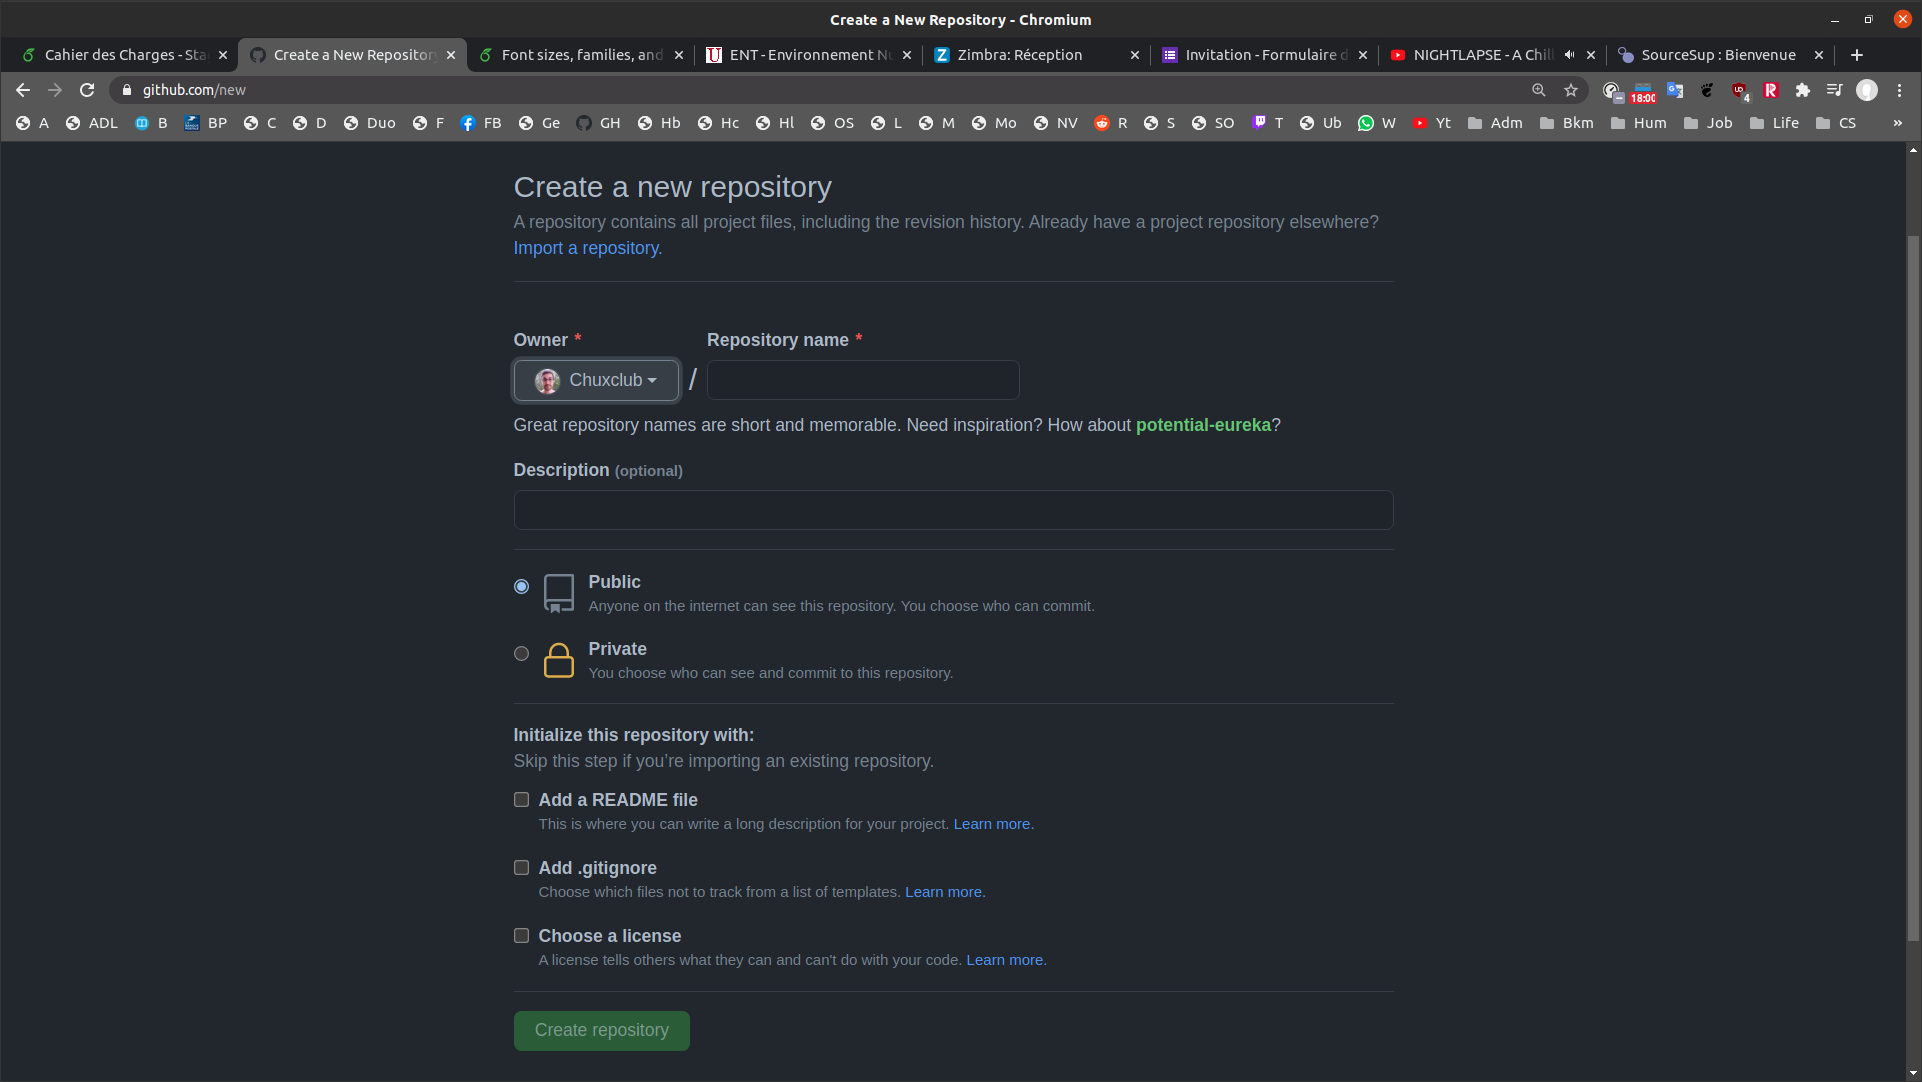
\includegraphics[scale=0.15]{github_createRepo.png}
\end{center}
\end{frame}

\begin{frame}{Régler la visibilité après la création du dépôt}
\begin{center}
	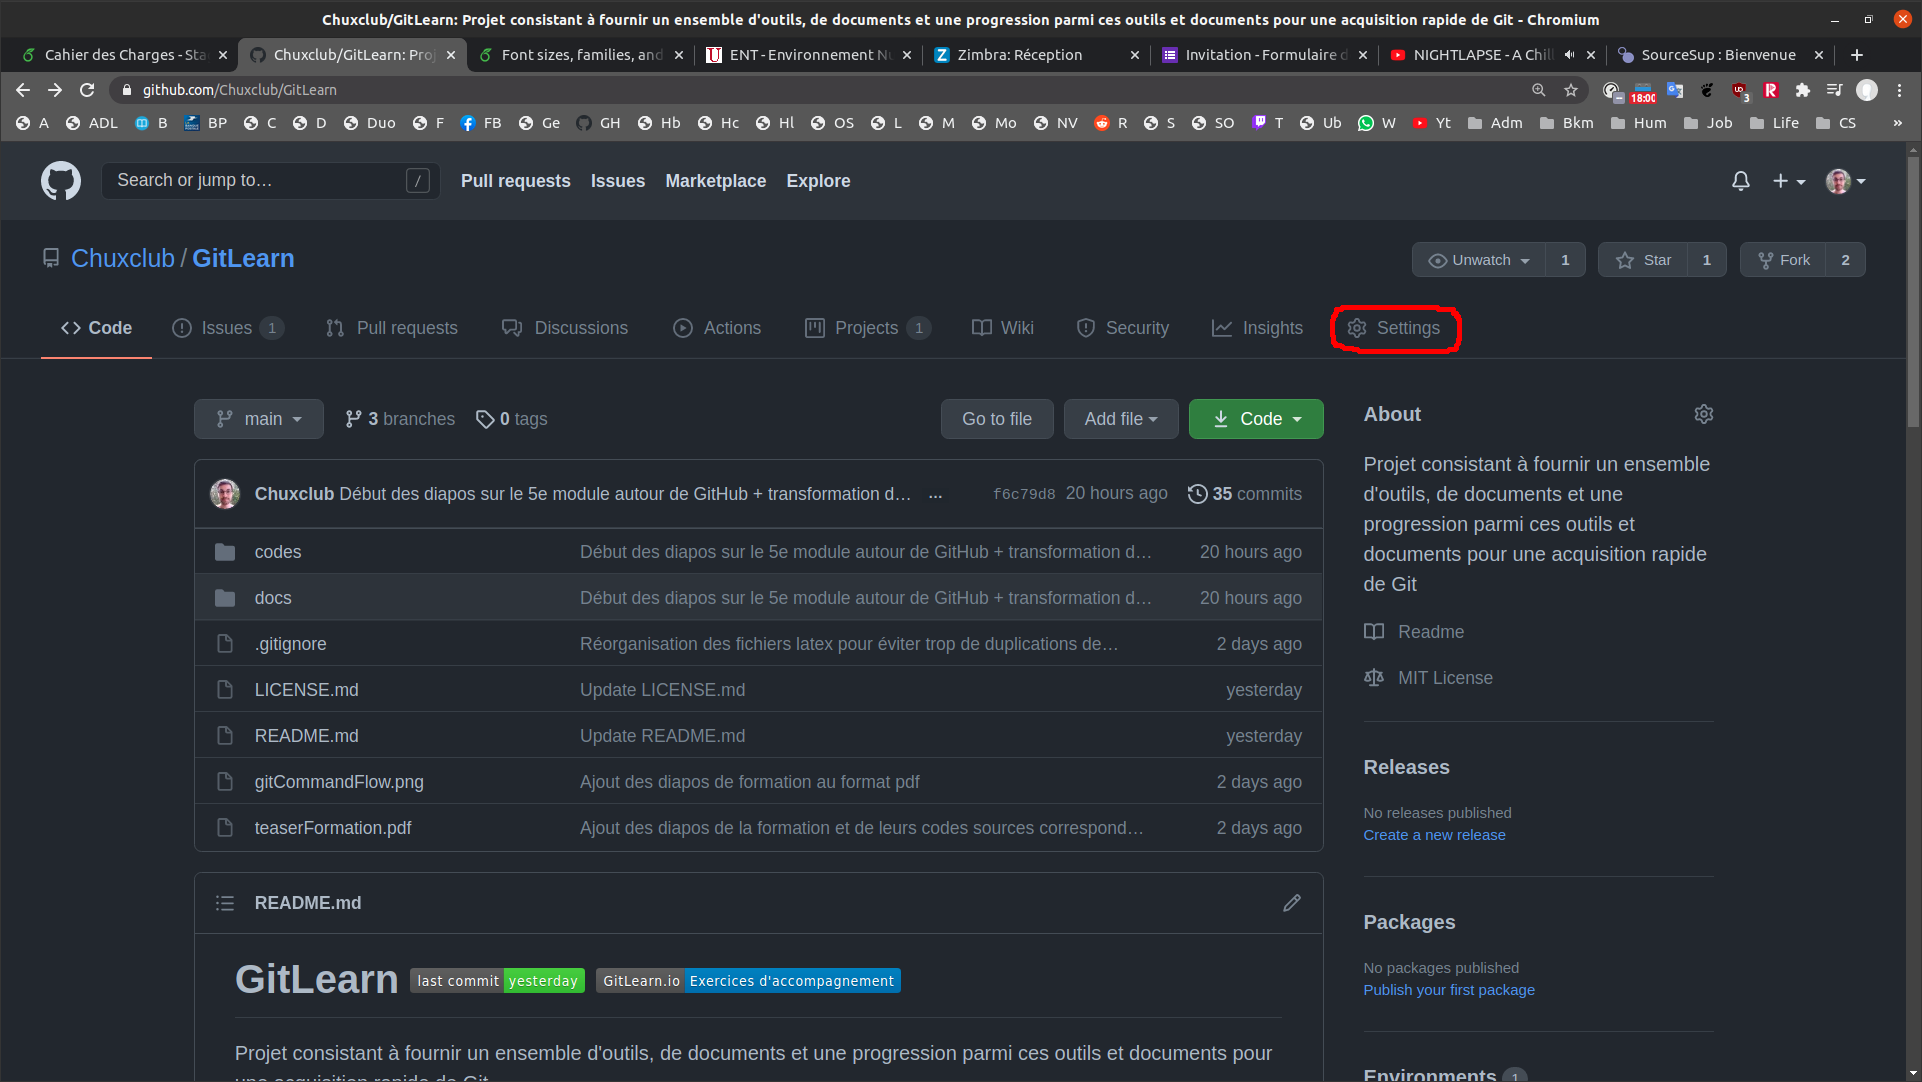
\includegraphics[scale=0.15]{github_settings_E.png}
\end{center}
\end{frame}

\begin{frame}{Régler la visibilité après la création du dépôt}
\begin{center}
	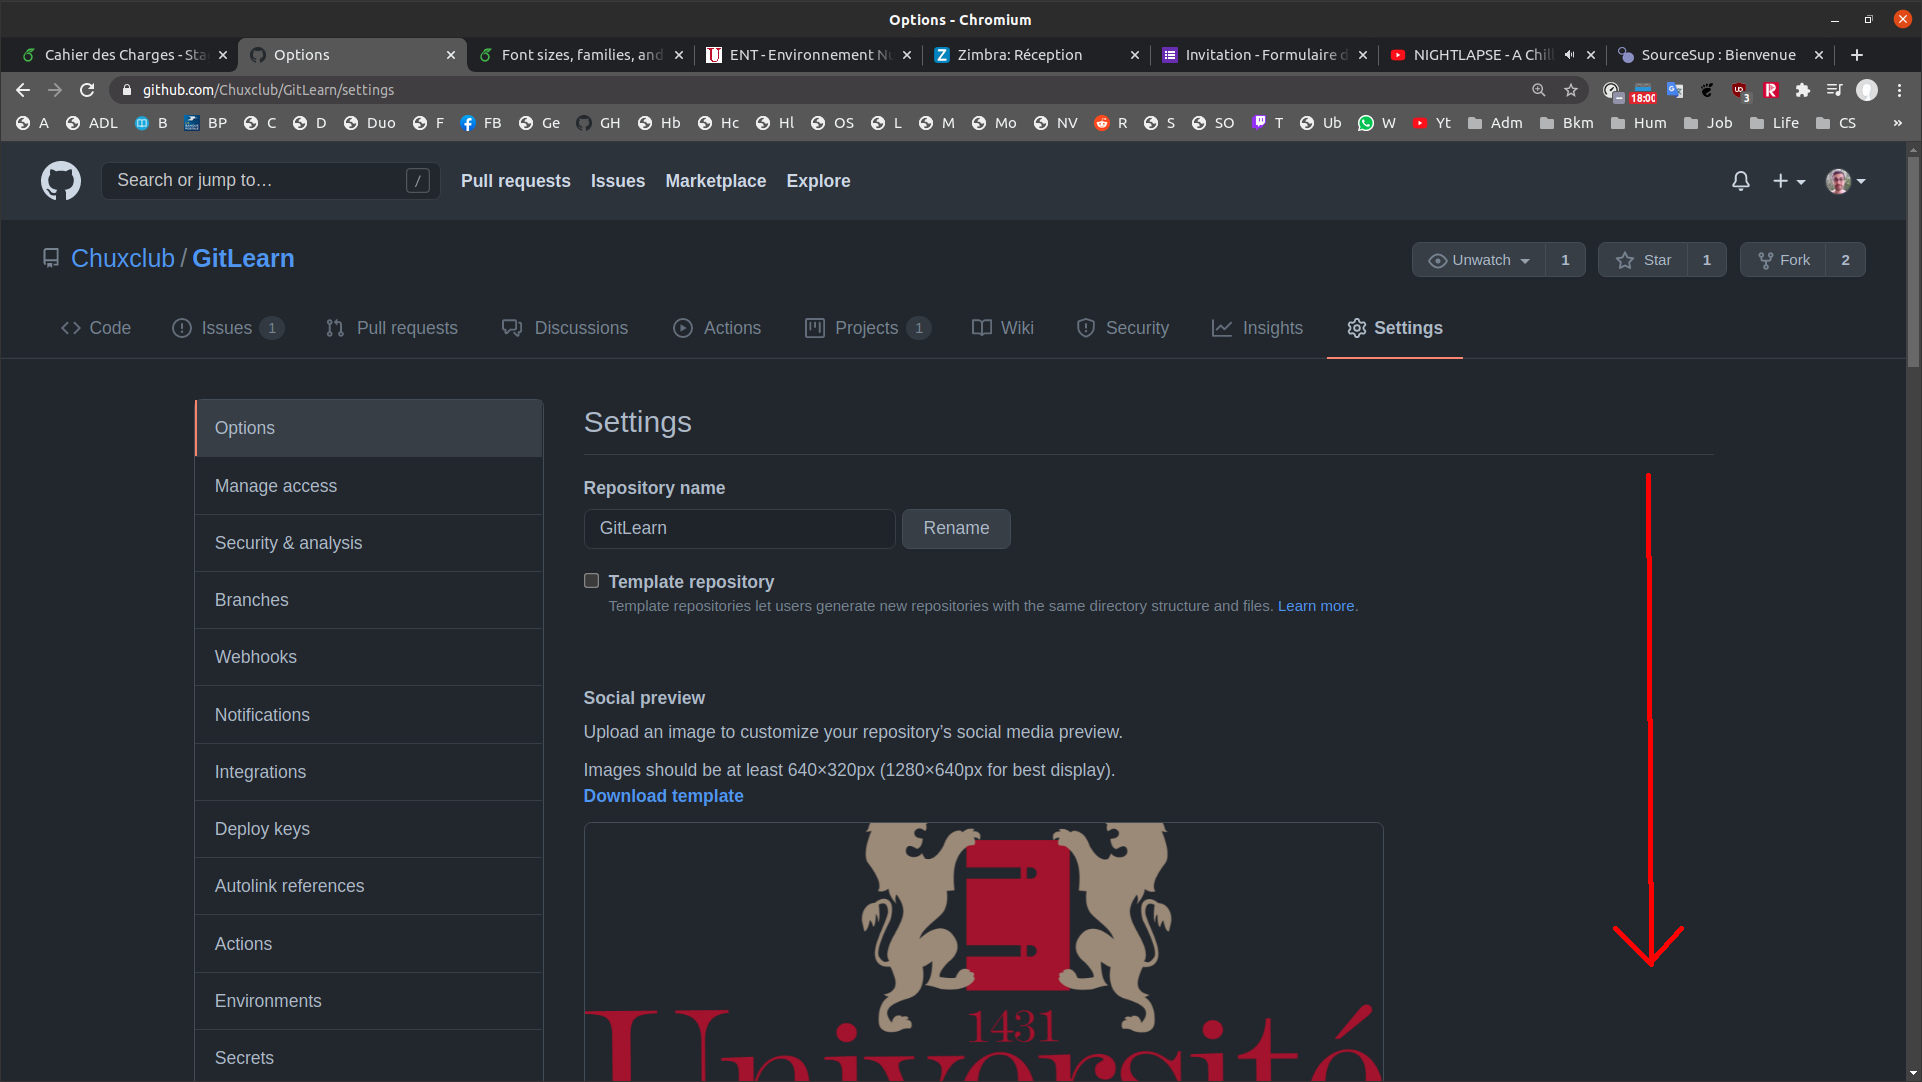
\includegraphics[scale=0.15]{github_options_E.png}
\end{center}
\end{frame}

\begin{frame}{Régler la visibilité après la création du dépôt}
\begin{center}
	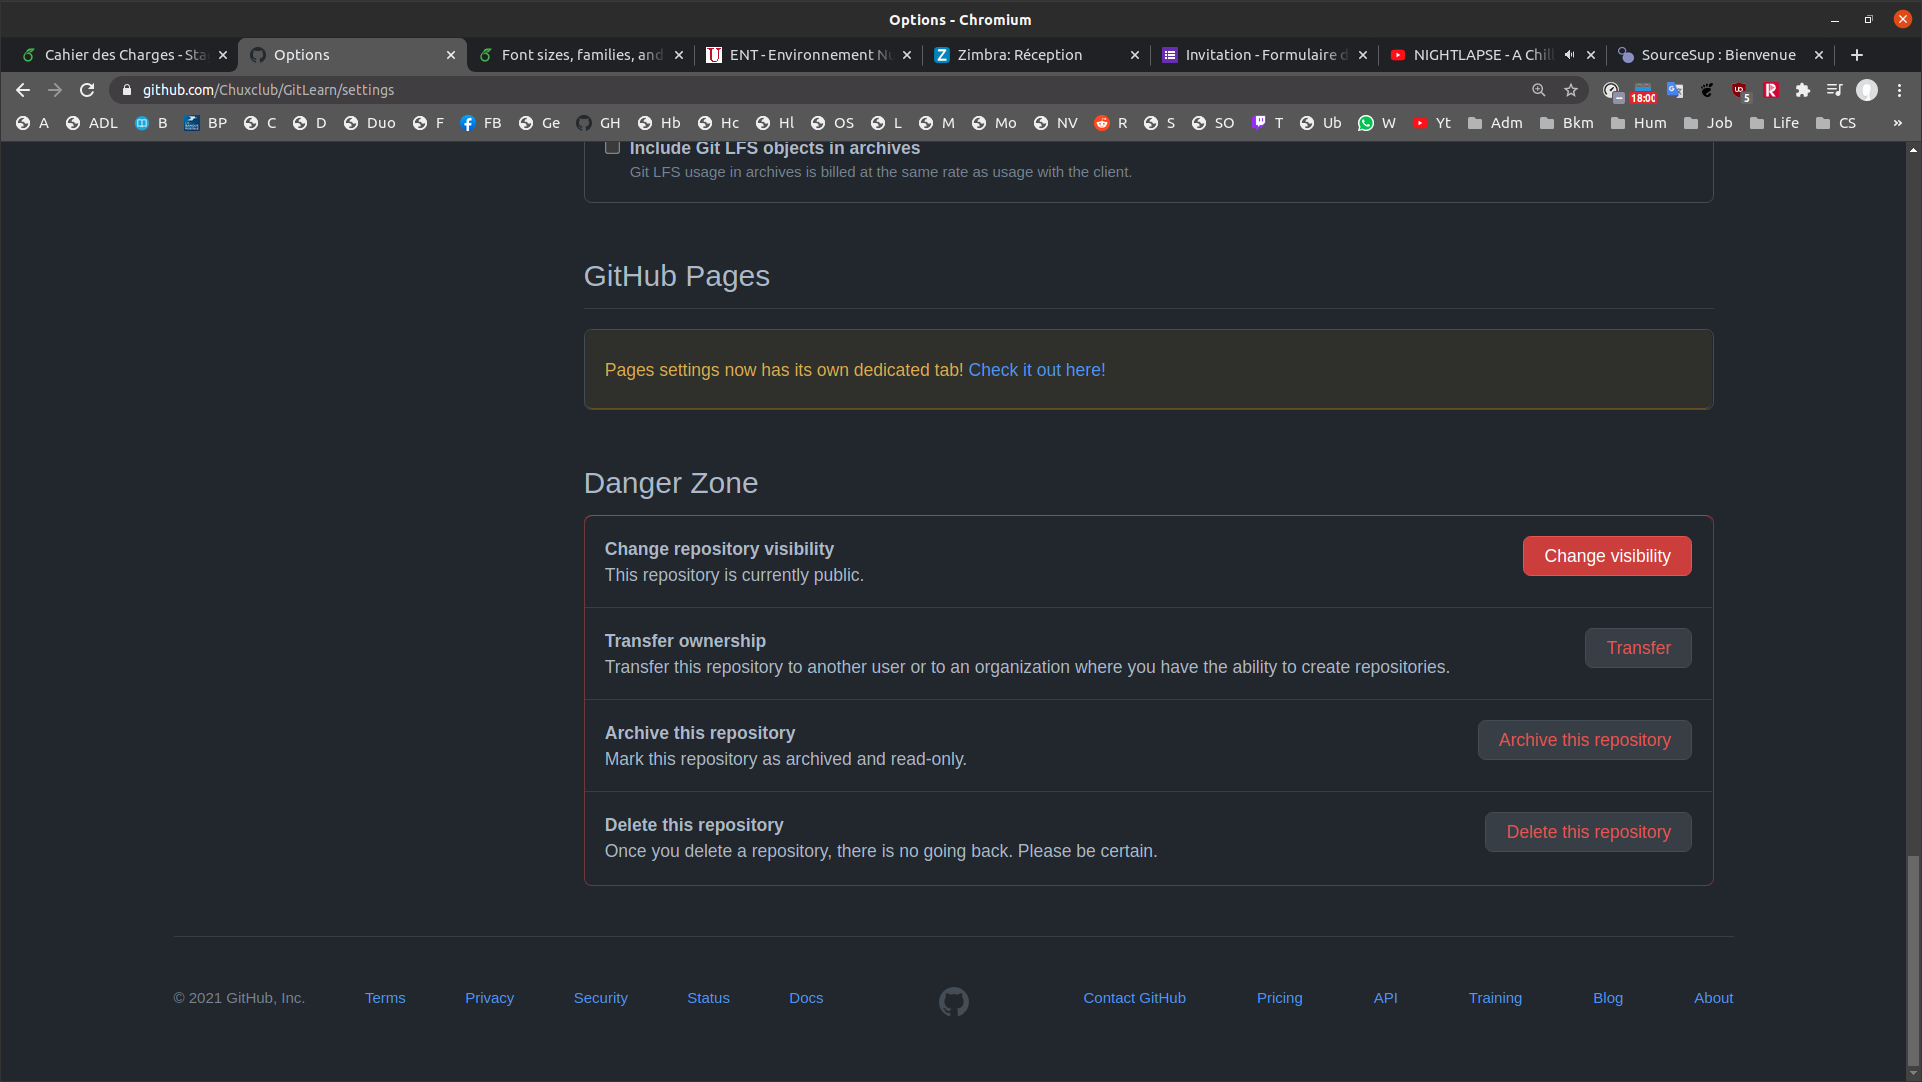
\includegraphics[scale=0.15]{github_visibility.png}
\end{center}
\end{frame}

% Subsection:
\subsection{Collaborer}
\begin{frame}{Inviter un collaborateur}
Il y a trois scénarios possibles, qui dépendent de la configuration du ou des dépôts distants.
\medskip

\underline{Premier scénario:}\\
\smallskip
Vous êtes indiqué comme \textbf{collaborateur} sur la branche distante. En tant que collaborateur vous pouvez "pusher" les changements que vous voulez sans restriction ! Sauf si le projet fait partie d'une organisation...\\
\medskip
\textbf{ATTENTION pour les chefs de projet:} Cela nécessite d'avoir une très grande confiance en ses collaborateurs. En cas de doute une des solutions est alors d'avoir une branche distante de développement
\end{frame}

\begin{frame}{Inviter un collaborateur}

\begin{center}
\begin{figure}[h!]
    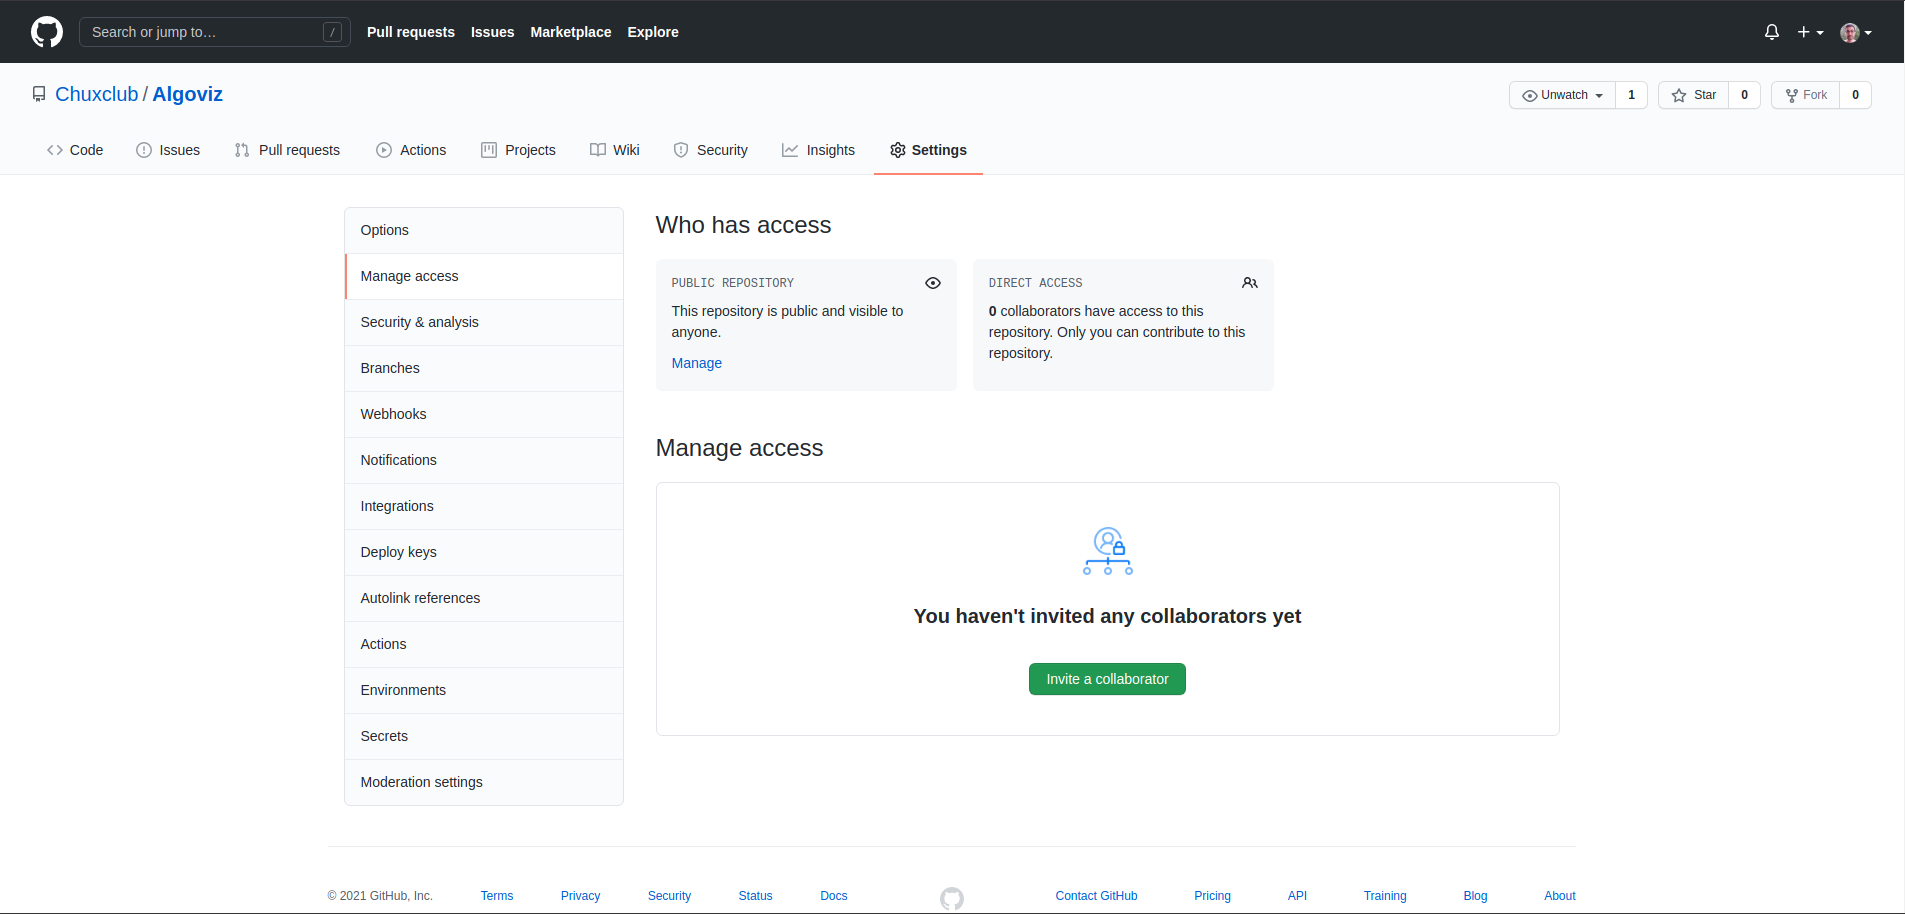
\includegraphics[scale=0.15]{images/droits_push/collaborator.png}
    \caption{Définir des collaborateurs sous GitHub}
\end{figure}
\end{center}

\end{frame}

\begin{frame}{Fork et Pull request}

\underline{Second scénario:}\\
\smallskip

\begin{enumerate}
    \item Vous avez "\textbf{forké}" (càd copié) sous Github le projet d'une personne.
    \item Vous avez ensuite cloné ce fork.
    \item Vous avez travaillé sur ce clone et "pushé" vos projets sur votre fork distant.
    \item Vous pouvez ensuite faire un pull request directement sur l'interface GitHub.
\end{enumerate}

\normalsize
\end{frame}

\begin{frame}{Fork et Pull request}
\begin{figure}[h!]
    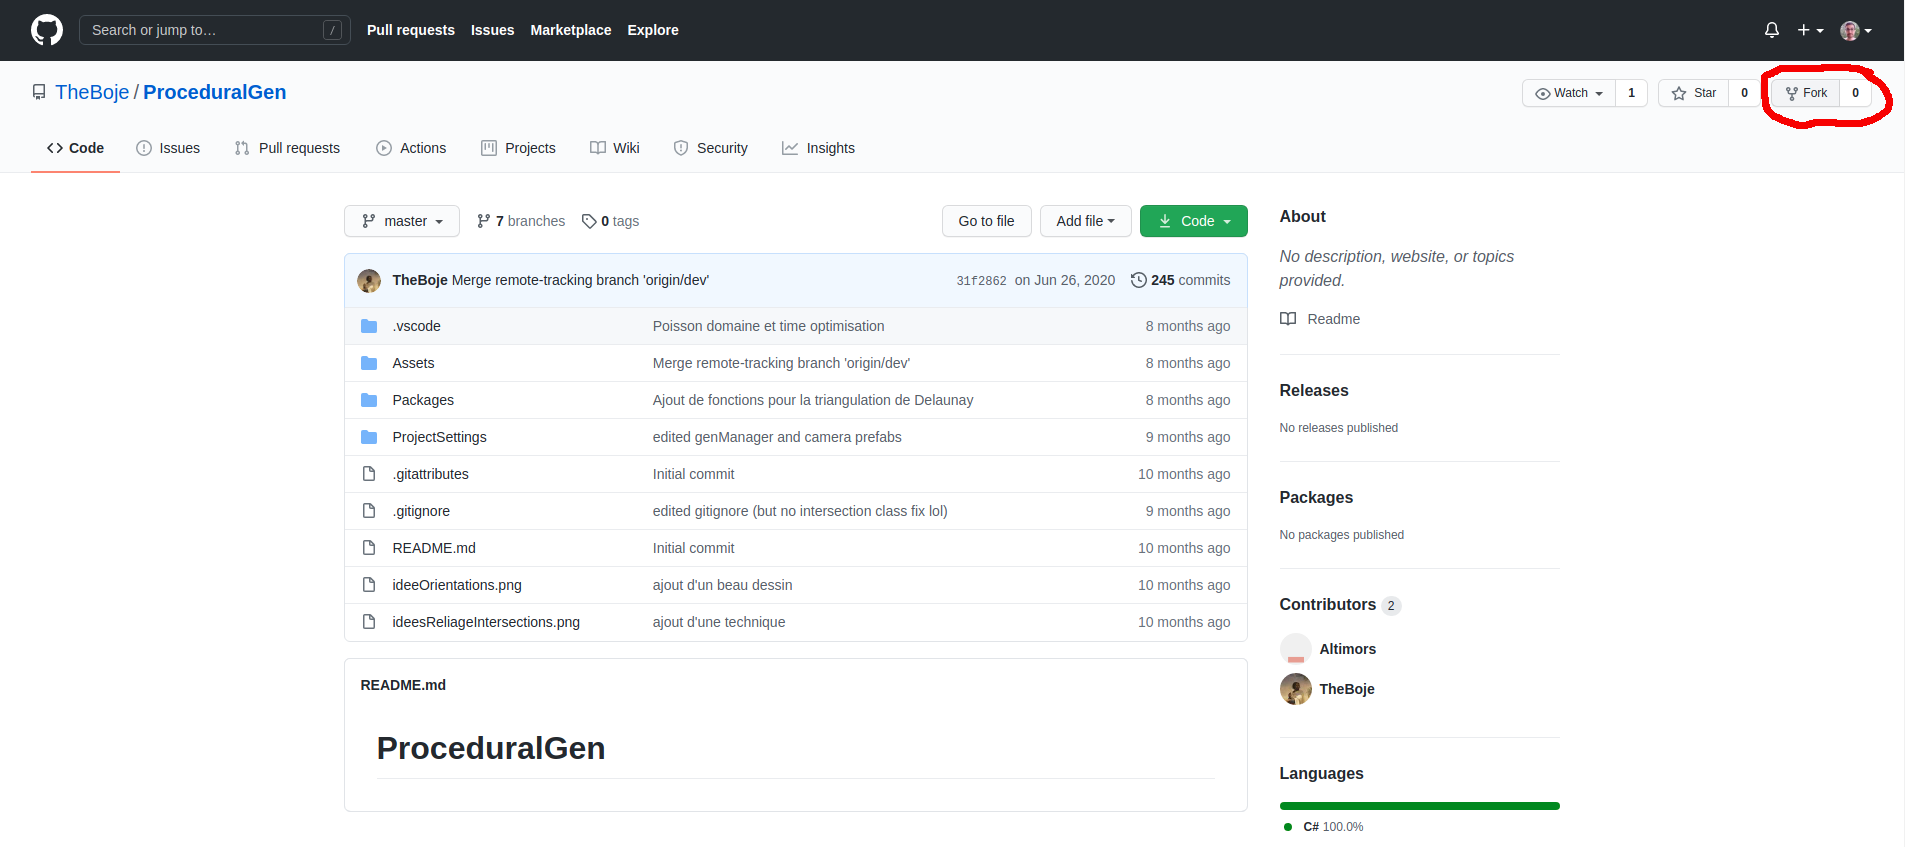
\includegraphics[scale=0.15]{images/droits_push/fork.png}
    \caption{Forker sous GitHub}
\end{figure}
\end{frame}

\begin{frame}{Fork et Pull request}
\begin{figure}[h!]
    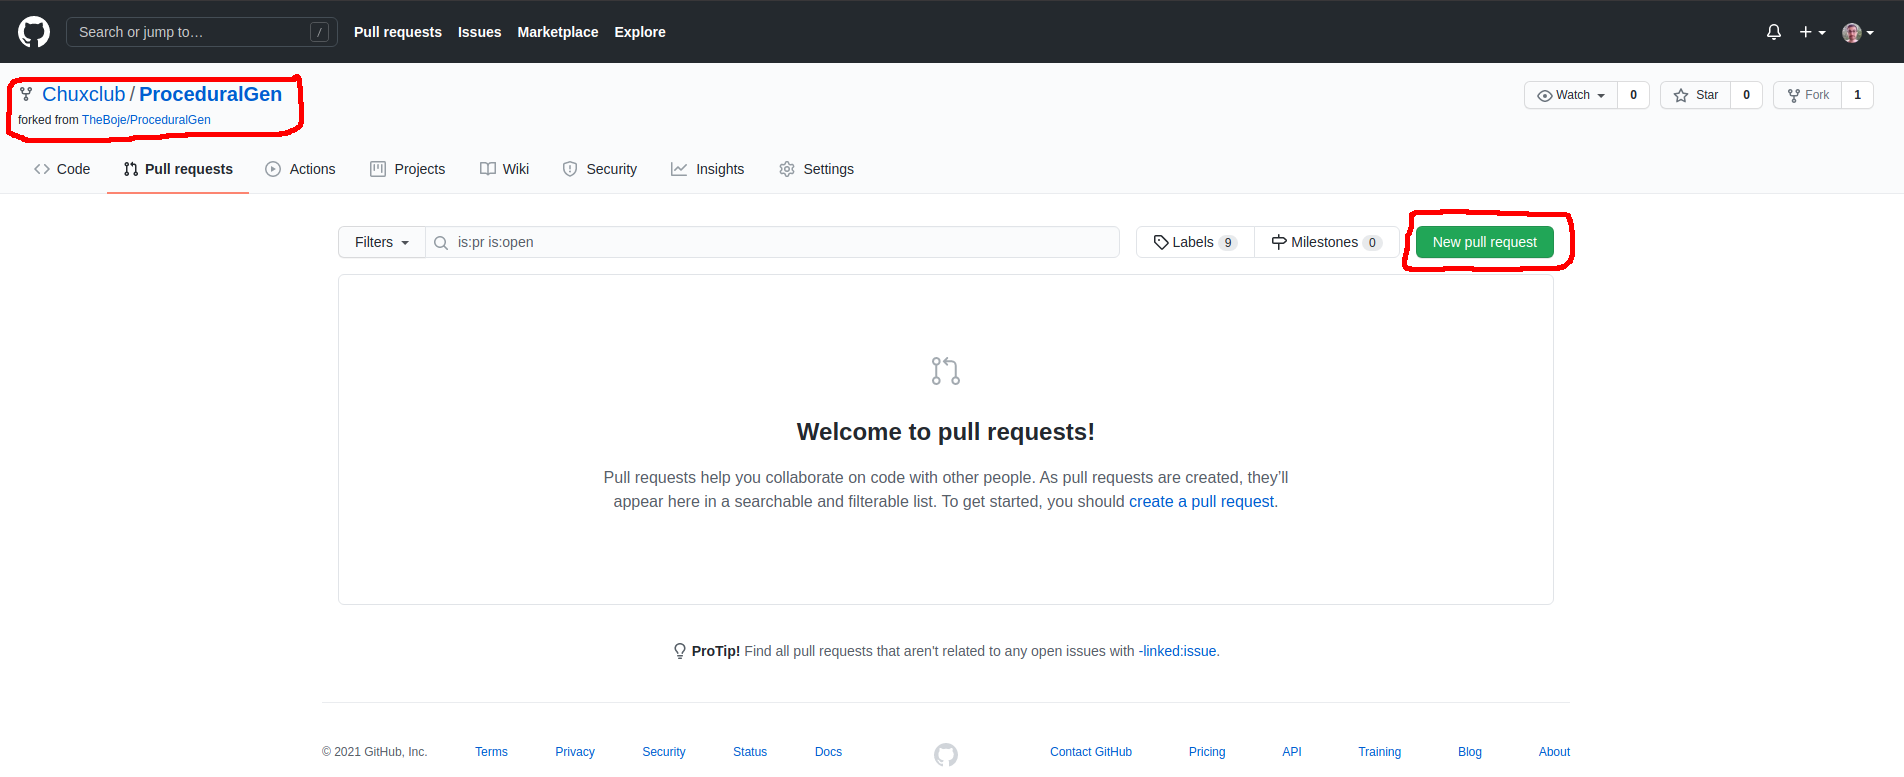
\includegraphics[scale=0.15]{images/droits_push/pull_request.png}
    \caption{Faire un pull request sous GitHub}
\end{figure}
\end{frame}


\begin{frame}{Fork tardif}

\underline{Dernier scénario:}\\
\smallskip
Vous avez \textbf{cloné} le projet d'une personne. Vous avez ensuite travaillé dessus et vous vous rendez compte que vous souhaiteriez faire part de vos modifications à l'auteur...\\
\medskip

\begin{enumerate}
    \item Comme précédemment vous forkez
    \item Vous ajoutez une branche distante à votre clone: "git remote add <nom> <urlDeVotreDepot>" ou, plus brutal: "git remote rm origin" suivi de "git remote add origin <urlDeVotreDepot>"
    \item Vous pushez vos changements sur ce fork
    \item Vous faites un pull request comme précédemment
\end{enumerate}
\end{frame}




%% --------------------- %%
%%        SECTION        %%
%% --------------------- %%
\AtBeginSection[]
{
  \begin{frame}
    \frametitle{Table of Contents}
    \tableofcontents[sectionstyle=show/hide,subsectionstyle=show/show/hide]
  \end{frame}
}


\section{Communiquer autour du projet avec GitHub}


% Subsection:
\subsection{Communiquer}
\begin{frame}{}
\end{frame}


% Subsection:
\subsection{Les fichiers spéciaux}
\begin{frame}{}
\end{frame}


% Subsection:
\subsection{La syntaxe MarkDown}
\begin{frame}{}
\end{frame}



%% --------------------- %%
%%        SECTION        %%
%% --------------------- %%
\AtBeginSection[]
{
  \begin{frame}
    \frametitle{Table of Contents}
    \tableofcontents[sectionstyle=show/hide,subsectionstyle=show/show/hide]
  \end{frame}
}


\section{Pour aller plus loin avec GitHub}


% Subsection:
\subsection{Le README de son profil}
\begin{frame}{}
\end{frame}


% Subsection:
\subsection{Les Shields en tête du README}
\begin{frame}{}
\end{frame}


% Subsection:
\subsection{Les organisations}
\begin{frame}{}
\end{frame}


% Subsection:
\subsection{Les logiciels avec une API GitHub}
\begin{frame}{}
\end{frame}


\end{document}